% Options for packages loaded elsewhere
% Options for packages loaded elsewhere
\PassOptionsToPackage{unicode}{hyperref}
\PassOptionsToPackage{hyphens}{url}
\PassOptionsToPackage{dvipsnames,svgnames,x11names}{xcolor}
%
\documentclass[
  letterpaper,
  DIV=11,
  numbers=noendperiod]{scrartcl}
\usepackage{xcolor}
\usepackage{amsmath,amssymb}
\setcounter{secnumdepth}{-\maxdimen} % remove section numbering
\usepackage{iftex}
\ifPDFTeX
  \usepackage[T1]{fontenc}
  \usepackage[utf8]{inputenc}
  \usepackage{textcomp} % provide euro and other symbols
\else % if luatex or xetex
  \usepackage{unicode-math} % this also loads fontspec
  \defaultfontfeatures{Scale=MatchLowercase}
  \defaultfontfeatures[\rmfamily]{Ligatures=TeX,Scale=1}
\fi
\usepackage{lmodern}
\ifPDFTeX\else
  % xetex/luatex font selection
\fi
% Use upquote if available, for straight quotes in verbatim environments
\IfFileExists{upquote.sty}{\usepackage{upquote}}{}
\IfFileExists{microtype.sty}{% use microtype if available
  \usepackage[]{microtype}
  \UseMicrotypeSet[protrusion]{basicmath} % disable protrusion for tt fonts
}{}
\makeatletter
\@ifundefined{KOMAClassName}{% if non-KOMA class
  \IfFileExists{parskip.sty}{%
    \usepackage{parskip}
  }{% else
    \setlength{\parindent}{0pt}
    \setlength{\parskip}{6pt plus 2pt minus 1pt}}
}{% if KOMA class
  \KOMAoptions{parskip=half}}
\makeatother
% Make \paragraph and \subparagraph free-standing
\makeatletter
\ifx\paragraph\undefined\else
  \let\oldparagraph\paragraph
  \renewcommand{\paragraph}{
    \@ifstar
      \xxxParagraphStar
      \xxxParagraphNoStar
  }
  \newcommand{\xxxParagraphStar}[1]{\oldparagraph*{#1}\mbox{}}
  \newcommand{\xxxParagraphNoStar}[1]{\oldparagraph{#1}\mbox{}}
\fi
\ifx\subparagraph\undefined\else
  \let\oldsubparagraph\subparagraph
  \renewcommand{\subparagraph}{
    \@ifstar
      \xxxSubParagraphStar
      \xxxSubParagraphNoStar
  }
  \newcommand{\xxxSubParagraphStar}[1]{\oldsubparagraph*{#1}\mbox{}}
  \newcommand{\xxxSubParagraphNoStar}[1]{\oldsubparagraph{#1}\mbox{}}
\fi
\makeatother


\usepackage{longtable,booktabs,array}
\newcounter{none} % for unnumbered tables
\usepackage{calc} % for calculating minipage widths
% Correct order of tables after \paragraph or \subparagraph
\usepackage{etoolbox}
\makeatletter
\patchcmd\longtable{\par}{\if@noskipsec\mbox{}\fi\par}{}{}
\makeatother
% Allow footnotes in longtable head/foot
\IfFileExists{footnotehyper.sty}{\usepackage{footnotehyper}}{\usepackage{footnote}}
\makesavenoteenv{longtable}
\usepackage{graphicx}
\makeatletter
\newsavebox\pandoc@box
\newcommand*\pandocbounded[1]{% scales image to fit in text height/width
  \sbox\pandoc@box{#1}%
  \Gscale@div\@tempa{\textheight}{\dimexpr\ht\pandoc@box+\dp\pandoc@box\relax}%
  \Gscale@div\@tempb{\linewidth}{\wd\pandoc@box}%
  \ifdim\@tempb\p@<\@tempa\p@\let\@tempa\@tempb\fi% select the smaller of both
  \ifdim\@tempa\p@<\p@\scalebox{\@tempa}{\usebox\pandoc@box}%
  \else\usebox{\pandoc@box}%
  \fi%
}
% Set default figure placement to htbp
\def\fps@figure{htbp}
\makeatother





\setlength{\emergencystretch}{3em} % prevent overfull lines

\providecommand{\tightlist}{%
  \setlength{\itemsep}{0pt}\setlength{\parskip}{0pt}}



 


\KOMAoption{captions}{tableheading}
\makeatletter
\@ifpackageloaded{caption}{}{\usepackage{caption}}
\AtBeginDocument{%
\ifdefined\contentsname
  \renewcommand*\contentsname{Table of contents}
\else
  \newcommand\contentsname{Table of contents}
\fi
\ifdefined\listfigurename
  \renewcommand*\listfigurename{List of Figures}
\else
  \newcommand\listfigurename{List of Figures}
\fi
\ifdefined\listtablename
  \renewcommand*\listtablename{List of Tables}
\else
  \newcommand\listtablename{List of Tables}
\fi
\ifdefined\figurename
  \renewcommand*\figurename{Figure}
\else
  \newcommand\figurename{Figure}
\fi
\ifdefined\tablename
  \renewcommand*\tablename{Table}
\else
  \newcommand\tablename{Table}
\fi
}
\@ifpackageloaded{float}{}{\usepackage{float}}
\floatstyle{ruled}
\@ifundefined{c@chapter}{\newfloat{codelisting}{h}{lop}}{\newfloat{codelisting}{h}{lop}[chapter]}
\floatname{codelisting}{Listing}
\newcommand*\listoflistings{\listof{codelisting}{List of Listings}}
\makeatother
\makeatletter
\makeatother
\makeatletter
\@ifpackageloaded{caption}{}{\usepackage{caption}}
\@ifpackageloaded{subcaption}{}{\usepackage{subcaption}}
\makeatother
\usepackage{bookmark}
\IfFileExists{xurl.sty}{\usepackage{xurl}}{} % add URL line breaks if available
\urlstyle{same}
% fallback for those not using the hyperref driver hyperxmp:
\makeatletter
\@ifundefined{xmpquote}{\newcommand{\xmpquote}[1]{#1}}{}
\makeatother
\hypersetup{
  pdftitle={Formula sheet},
  colorlinks=true,
  linkcolor={blue},
  filecolor={Maroon},
  citecolor={Blue},
  urlcolor={Blue},
  pdfcreator={LaTeX via pandoc}}


\title{Formula sheet}
\author{}
\date{}
\begin{document}
\maketitle


\subsection{General Part}\label{general-part}

Mean: \(\bar{X} = \frac{\Sigma_{i=1}^nx_i}{N}\)

Variance: \(S^2_x = \frac{\Sigma_{i=1}^n(x_i-\bar{x})^2}{n-1}\)

Standardized values (Z-values): \(Z = \frac{X-\mu}{\sigma}\)

Z-statistic in one sample Z-test:
\(Z = \frac{\bar{x}-\mu_x}{\sigma_{x}}\)

Standard error of the mean:
\(\sigma_{\bar{x}} = \frac{\sigma}{\sqrt{n}}\)

Cohen's d: \(\frac{\bar{X}_1-\bar{X}_2}{s_{pooled}}\)

\(s^2_{pooled} = \frac{(n_1-1)*s_1^2 + (n_2-1)*s_2^2}{n_1+n_2-2}\)

\(s_{pooled} = \sqrt{s^2_{pooled}}\)

\section{Z-table}\label{z-table}

Table gives the right-tail probability corresponding to a Z-value of the
value in the Z-column plus the value in the column name, which indicates
the second digit of the Z-score.

\pandocbounded{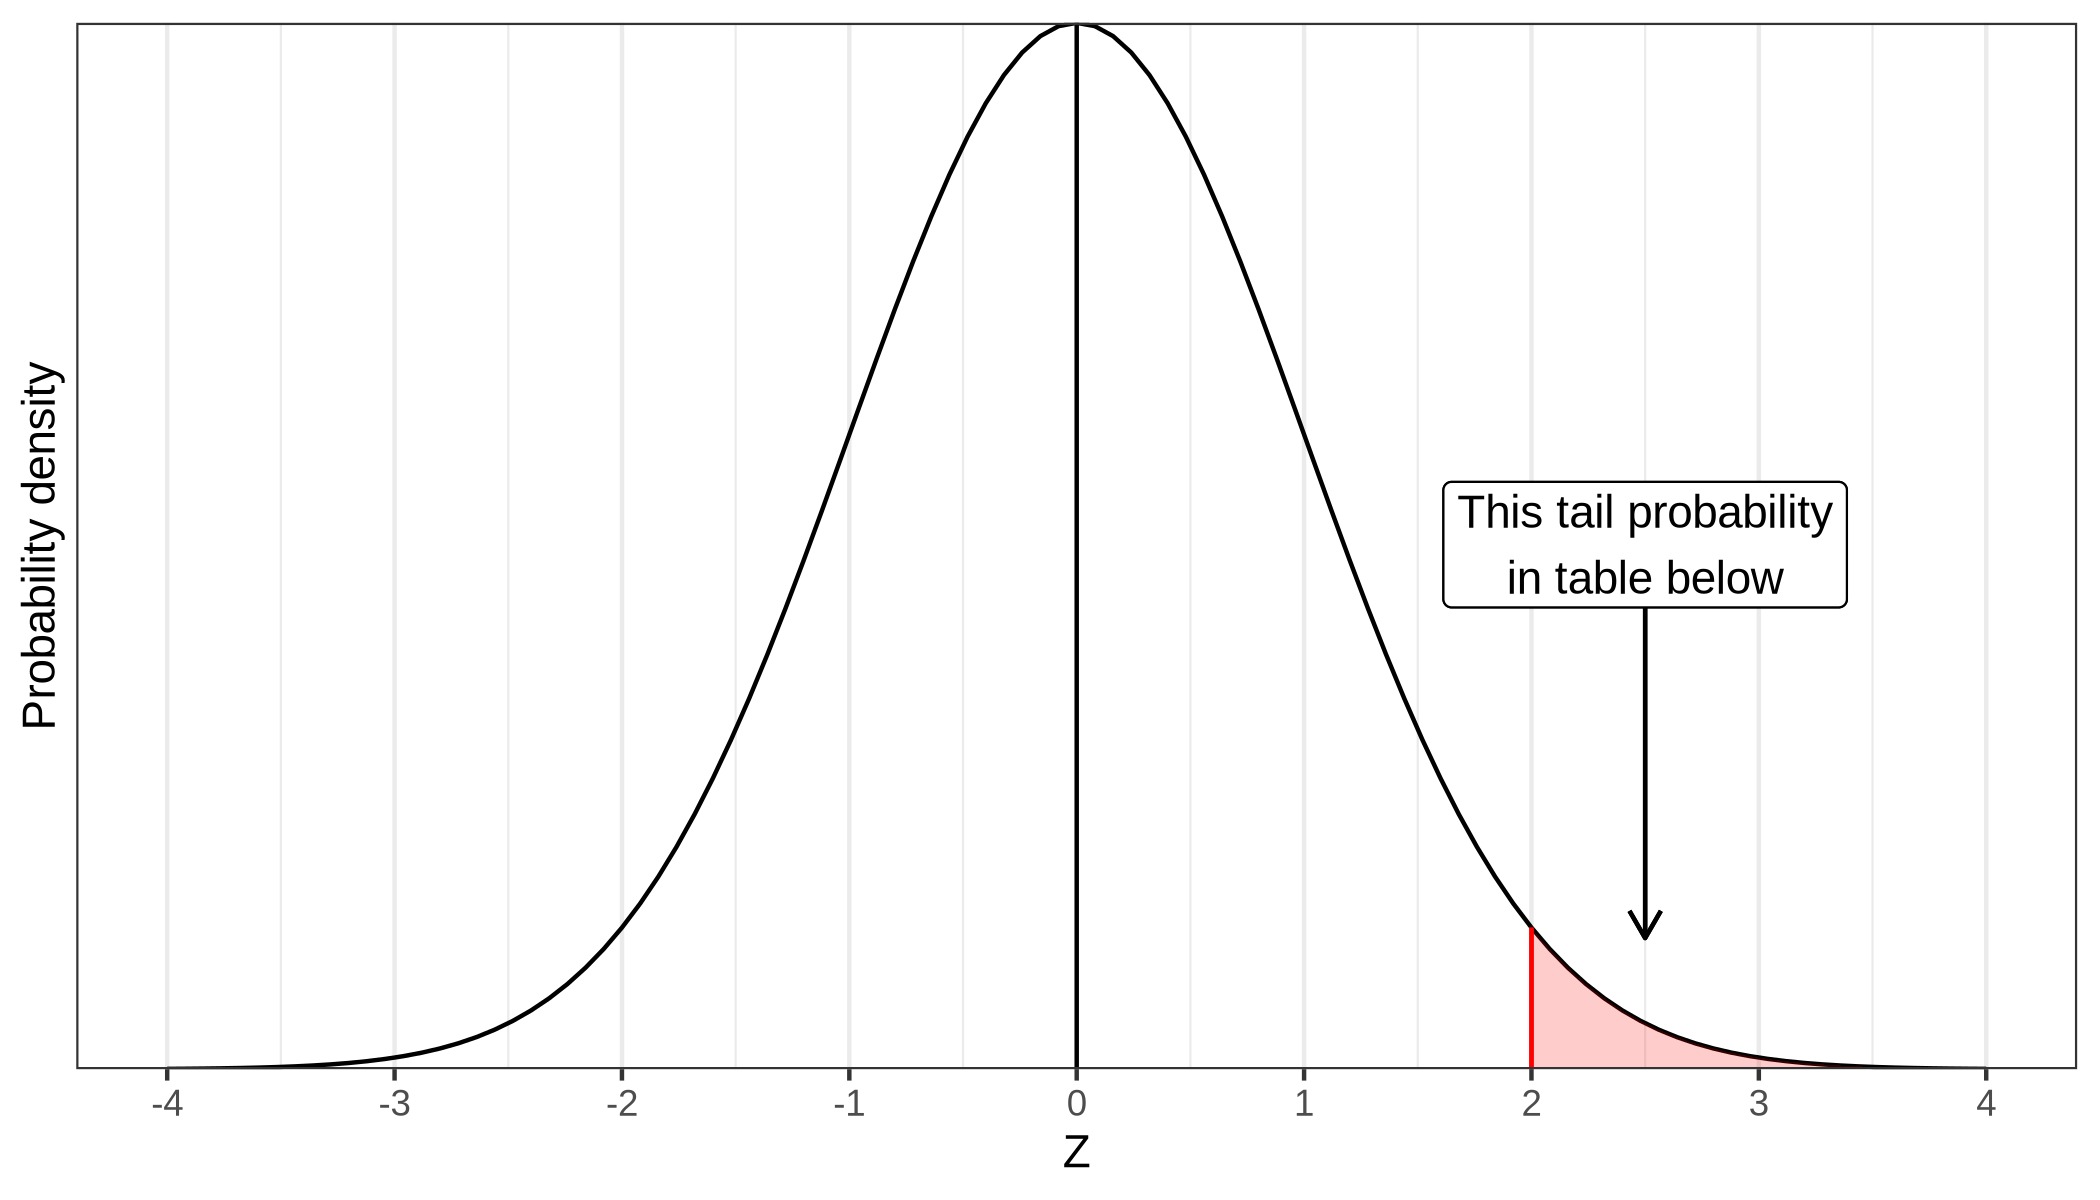
\includegraphics[keepaspectratio]{ztable.png}}

{\def\LTcaptype{none} % do not increment counter
\begin{longtable}[]{@{}
  >{\raggedright\arraybackslash}p{(\linewidth - 20\tabcolsep) * \real{0.0625}}
  >{\raggedleft\arraybackslash}p{(\linewidth - 20\tabcolsep) * \real{0.0938}}
  >{\raggedleft\arraybackslash}p{(\linewidth - 20\tabcolsep) * \real{0.0938}}
  >{\raggedleft\arraybackslash}p{(\linewidth - 20\tabcolsep) * \real{0.0938}}
  >{\raggedleft\arraybackslash}p{(\linewidth - 20\tabcolsep) * \real{0.0938}}
  >{\raggedleft\arraybackslash}p{(\linewidth - 20\tabcolsep) * \real{0.0938}}
  >{\raggedleft\arraybackslash}p{(\linewidth - 20\tabcolsep) * \real{0.0938}}
  >{\raggedleft\arraybackslash}p{(\linewidth - 20\tabcolsep) * \real{0.0938}}
  >{\raggedleft\arraybackslash}p{(\linewidth - 20\tabcolsep) * \real{0.0938}}
  >{\raggedleft\arraybackslash}p{(\linewidth - 20\tabcolsep) * \real{0.0938}}
  >{\raggedleft\arraybackslash}p{(\linewidth - 20\tabcolsep) * \real{0.0938}}@{}}
\toprule\noalign{}
\begin{minipage}[b]{\linewidth}\raggedright
Z
\end{minipage} & \begin{minipage}[b]{\linewidth}\raggedleft
0
\end{minipage} & \begin{minipage}[b]{\linewidth}\raggedleft
0.01
\end{minipage} & \begin{minipage}[b]{\linewidth}\raggedleft
0.02
\end{minipage} & \begin{minipage}[b]{\linewidth}\raggedleft
0.03
\end{minipage} & \begin{minipage}[b]{\linewidth}\raggedleft
0.04
\end{minipage} & \begin{minipage}[b]{\linewidth}\raggedleft
0.05
\end{minipage} & \begin{minipage}[b]{\linewidth}\raggedleft
0.06
\end{minipage} & \begin{minipage}[b]{\linewidth}\raggedleft
0.07
\end{minipage} & \begin{minipage}[b]{\linewidth}\raggedleft
0.08
\end{minipage} & \begin{minipage}[b]{\linewidth}\raggedleft
0.09
\end{minipage} \\
\midrule\noalign{}
\endhead
\bottomrule\noalign{}
\endlastfoot
0 & 0.500 & 0.496 & 0.492 & 0.488 & 0.484 & 0.480 & 0.476 & 0.472 &
0.468 & 0.464 \\
0.1 & 0.460 & 0.456 & 0.452 & 0.448 & 0.444 & 0.440 & 0.436 & 0.433 &
0.429 & 0.425 \\
0.2 & 0.421 & 0.417 & 0.413 & 0.409 & 0.405 & 0.401 & 0.397 & 0.394 &
0.390 & 0.386 \\
0.3 & 0.382 & 0.378 & 0.374 & 0.371 & 0.367 & 0.363 & 0.359 & 0.356 &
0.352 & 0.348 \\
0.4 & 0.345 & 0.341 & 0.337 & 0.334 & 0.330 & 0.326 & 0.323 & 0.319 &
0.316 & 0.312 \\
0.5 & 0.309 & 0.305 & 0.302 & 0.298 & 0.295 & 0.291 & 0.288 & 0.284 &
0.281 & 0.278 \\
0.6 & 0.274 & 0.271 & 0.268 & 0.264 & 0.261 & 0.258 & 0.255 & 0.251 &
0.248 & 0.245 \\
0.7 & 0.242 & 0.239 & 0.236 & 0.233 & 0.230 & 0.227 & 0.224 & 0.221 &
0.218 & 0.215 \\
0.8 & 0.212 & 0.209 & 0.206 & 0.203 & 0.200 & 0.198 & 0.195 & 0.192 &
0.189 & 0.187 \\
0.9 & 0.184 & 0.181 & 0.179 & 0.176 & 0.174 & 0.171 & 0.169 & 0.166 &
0.164 & 0.161 \\
1 & 0.159 & 0.156 & 0.154 & 0.152 & 0.149 & 0.147 & 0.145 & 0.142 &
0.140 & 0.138 \\
1.1 & 0.136 & 0.133 & 0.131 & 0.129 & 0.127 & 0.125 & 0.123 & 0.121 &
0.119 & 0.117 \\
1.2 & 0.115 & 0.113 & 0.111 & 0.109 & 0.107 & 0.106 & 0.104 & 0.102 &
0.100 & 0.099 \\
1.3 & 0.097 & 0.095 & 0.093 & 0.092 & 0.090 & 0.089 & 0.087 & 0.085 &
0.084 & 0.082 \\
1.4 & 0.081 & 0.079 & 0.078 & 0.076 & 0.075 & 0.074 & 0.072 & 0.071 &
0.069 & 0.068 \\
1.5 & 0.067 & 0.066 & 0.064 & 0.063 & 0.062 & 0.061 & 0.059 & 0.058 &
0.057 & 0.056 \\
1.6 & 0.055 & 0.054 & 0.053 & 0.052 & 0.051 & 0.049 & 0.048 & 0.047 &
0.046 & 0.046 \\
1.7 & 0.045 & 0.044 & 0.043 & 0.042 & 0.041 & 0.040 & 0.039 & 0.038 &
0.038 & 0.037 \\
1.8 & 0.036 & 0.035 & 0.034 & 0.034 & 0.033 & 0.032 & 0.031 & 0.031 &
0.030 & 0.029 \\
1.9 & 0.029 & 0.028 & 0.027 & 0.027 & 0.026 & 0.026 & 0.025 & 0.024 &
0.024 & 0.023 \\
2 & 0.023 & 0.022 & 0.022 & 0.021 & 0.021 & 0.020 & 0.020 & 0.019 &
0.019 & 0.018 \\
2.1 & 0.018 & 0.017 & 0.017 & 0.017 & 0.016 & 0.016 & 0.015 & 0.015 &
0.015 & 0.014 \\
2.2 & 0.014 & 0.014 & 0.013 & 0.013 & 0.013 & 0.012 & 0.012 & 0.012 &
0.011 & 0.011 \\
2.3 & 0.011 & 0.010 & 0.010 & 0.010 & 0.010 & 0.009 & 0.009 & 0.009 &
0.009 & 0.008 \\
2.4 & 0.008 & 0.008 & 0.008 & 0.008 & 0.007 & 0.007 & 0.007 & 0.007 &
0.007 & 0.006 \\
2.5 & 0.006 & 0.006 & 0.006 & 0.006 & 0.006 & 0.005 & 0.005 & 0.005 &
0.005 & 0.005 \\
2.6 & 0.005 & 0.005 & 0.004 & 0.004 & 0.004 & 0.004 & 0.004 & 0.004 &
0.004 & 0.004 \\
2.7 & 0.003 & 0.003 & 0.003 & 0.003 & 0.003 & 0.003 & 0.003 & 0.003 &
0.003 & 0.003 \\
2.8 & 0.003 & 0.002 & 0.002 & 0.002 & 0.002 & 0.002 & 0.002 & 0.002 &
0.002 & 0.002 \\
2.9 & 0.002 & 0.002 & 0.002 & 0.002 & 0.002 & 0.002 & 0.002 & 0.001 &
0.001 & 0.001 \\
3 & 0.001 & 0.001 & 0.001 & 0.001 & 0.001 & 0.001 & 0.001 & 0.001 &
0.001 & 0.001 \\
\end{longtable}
}




\end{document}
